\chapter{Rendering Pipeline}
\begin{figure}[h]
	\centering
	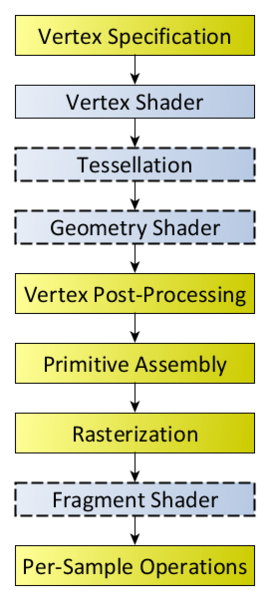
\includegraphics[scale=0.4]{imagens/openglPipeline.png}
	\caption{\small \textit{Rendering pipeline} OpenGL (Fonte: OpenGL, 2016)}
	\label{fig:glpipeline}
\end{figure}

O processo de execução de um programa que exibe resultados em um monitor gráfico requer uma série de etapas, com grande quantidade de cálculos (CLEMENTS, 2014). Assim como na CPU (\textit{Central Processing Unit}, Unidade de Processamento Central), que realiza o processamento geral do computador, a GPU (\textit{Graphics Processing Unit}, Unidade de Processamento Gráfico), também se beneficia de \textit{pipeline}.

Tal processo é definido pela execução paralela de múltiplas etapas, diminuindo a ociosidade do \textit{hardware} e aumentando a taxa de saída de dados (\textit{throuput}) (SHEN e LIPASTI, 2013). Logo que uma primeira instrução é finalizada em uma etapa, uma segunda pode iniciar, desde que não possua outras dependências.

A primeira etapa programável de processamento é o \textit{vertex shader}, sendo também a única obrigatória. Sua função é efetuar cálculos, tendo apenas um vértice como entrada e saída de dados (OpenGL, 2016b). Para funcionar corretamente, o programador deve especificar a entrada, chamada de \textit{vertex attribute}.

\begin{lstlisting}[language=glsl,
label={lst:vertexshader},
caption="Exemplo de \textit{vertex shader}"]
	#version 330
	layout (location = 0) in vec3 position;
	layout (location = 1) in vec3 normal;
	
	out vec3 Normal;
	out vec3 FragPos;
	
	uniform mat4 model;
	uniform mat4 view;
	uniform mat4 projection;
	
	void main()
	{
		gl_Position = projection * view *  model * vec4(position, 1.0f);
		FragPos = vec3(model * vec4(position, 1.0f));
		Normal = mat3(transpose(inverse(model))) * normal;  
	} 
}
\end{lstlisting}

No código \ref{lst:vertexshader}, podemos notar as entradas definidas por \lstinline{layout(location = #)} e as saídas por \lstinline{out}, que serão utilizadas na próxima etapa do \textit{pipeline}. Devido a natureza independente dos vértices, estes podem ser processados paralelamente em alta velocidade, fazendo uso dos múltiplos núcleos da GPU (AKENINE-MÖLLER et al, 2016).